%% article.tex
%% V1.4b
%% 2015/08/26
%% by Michael Shell
%% see http://www.michaelshell.org/
%% for current contact information.
%%
%% This is a skeleton file demonstrating the use of IEEEtran.cls
%% (requires IEEEtran.cls version 1.8b or later) with an IEEE
%% journal paper.
%%
%% Support sites:
%% http://www.michaelshell.org/tex/ieeetran/
%% http://www.ctan.org/pkg/ieeetran
%% and
%% http://www.ieee.org/

%%*************************************************************************
%% Legal Notice:
%% This code is offered as-is without any warranty either expressed or
%% implied; without even the implied warranty of MERCHANTABILITY or
%% FITNESS FOR A PARTICULAR PURPOSE! 
%% User assumes all risk.
%% In no event shall the IEEE or any contributor to this code be liable for
%% any damages or losses, including, but not limited to, incidental,
%% consequential, or any other damages, resulting from the use or misuse
%% of any information contained here.
%%
%% All comments are the opinions of their respective authors and are not
%% necessarily endorsed by the IEEE.
%%
%% This work is distributed under the LaTeX Project Public License (LPPL)
%% ( http://www.latex-project.org/ ) version 1.3, and may be freely used,
%% distributed and modified. A copy of the LPPL, version 1.3, is included
%% in the base LaTeX documentation of all distributions of LaTeX released
%% 2003/12/01 or later.
%% Retain all contribution notices and credits.
%% ** Modified files should be clearly indicated as such, including  **
%% ** renaming them and changing author support contact information. **
%%*************************************************************************


% *** Authors should verify (and, if needed, correct) their LaTeX system  ***
% *** with the testflow diagnostic prior to trusting their LaTeX platform ***
% *** with production work. The IEEE's font choices and paper sizes can   ***
% *** trigger bugs that do not appear when using other class files.       ***                          ***
% The testflow support page is at:
% http://www.michaelshell.org/tex/testflow/

\documentclass[journal]{IEEEtran}

\usepackage{cite}

\usepackage[pdftex]{graphicx}
\graphicspath{ {./images/} }

%\usepackage{amsmath}

\usepackage{algorithm}
\usepackage{algpseudocode}

%\usepackage{array}

%\usepackage[caption=false,font=normalsize,labelfont=sf,textfont=sf]{subfig}

%\usepackage{fixltx2e}

%\usepackage{stfloats}

%\usepackage{dblfloatfix}

%\usepackage{url}

\usepackage{hyperref}

% correct bad hyphenation here
\hyphenation{op-tical net-works semi-conduc-tor}

\algdef{SE}[SUBALG]{Indent}{EndIndent}{}{\algorithmicend\ }%
\algtext*{Indent}
\algtext*{EndIndent}

\newcommand{\LineComment}[1]{\State \texttt{/* #1 */}}


\begin{document}
%
% paper title
% Titles are generally capitalized except for words such as a, an, and, as,
% at, but, by, for, in, nor, of, on, or, the, to and up, which are usually
% not capitalized unless they are the first or last word of the title.
% Line breaks \\ can be used within to get better formatting as desired.
% Do not put math or special symbols in the title.
\title{The Units of Permissionless Consensus: \\ Towards Mobile and Edge Computing}
%
%
% author names and IEEE memberships
% note positions of commas and non breaking spaces ( ~ ) LaTeX will not break
% a structure at a ~ so this keeps an author's name from being broken across
% two lines.
% use \thanks{} to gain access to the first footnote area
% a separate \thanks must be used for each paragraph as LaTeX2e's \thanks
% was not built to handle multiple paragraphs
%

\author{Eduardo Ribas Brito \\ eduardo.ribas.brito@ut.ee}

% note the % following the last \IEEEmembership and also \thanks - 
% these prevent an unwanted space from occurring between the last author name
% and the end of the author line. i.e., if you had this:
% 
% \author{....lastname \thanks{...} \thanks{...} }
%                     ^------------^------------^----Do not want these spaces!
%
% a space would be appended to the last name and could cause every name on that
% line to be shifted left slightly. This is one of those "LaTeX things". For
% instance, "\textbf{A} \textbf{B}" will typeset as "A B" not "AB". To get
% "AB" then you have to do: "\textbf{A}\textbf{B}"
% \thanks is no different in this regard, so shield the last } of each \thanks
% that ends a line with a % and do not let a space in before the next \thanks.
% Spaces after \IEEEmembership other than the last one are OK (and needed) as
% you are supposed to have spaces between the names. For what it is worth,
% this is a minor point as most people would not even notice if the said evil
% space somehow managed to creep in.



% The paper headers
% \markboth{Journal of \LaTeX\ Class Files,~Vol.~14, No.~8, August~2015}%
% {Shell \MakeLowercase{\textit{et al.}}: Bare Demo of IEEEtran.cls for IEEE Journals}
% The only time the second header will appear is for the odd numbered pages
% after the title page when using the twoside option.
% 
% *** Note that you probably will NOT want to include the author's ***
% *** name in the headers of peer review papers.                   ***
% You can use \ifCLASSOPTIONpeerreview for conditional compilation here if
% you desire.




% If you want to put a publisher's ID mark on the page you can do it like
% this:
%\IEEEpubid{0000--0000/00\$00.00~\copyright~2015 IEEE}
% Remember, if you use this you must call \IEEEpubidadjcol in the second
% column for its text to clear the IEEEpubid mark.



% use for special paper notices
%\IEEEspecialpapernotice{(Invited Paper)}




% make the title area
\maketitle

% As a general rule, do not put math, special symbols or citations
% in the abstract or keywords.
\begin{abstract}
...
\end{abstract}

% Note that keywords are not normally used for peer review papers.
\begin{IEEEkeywords}
IEEE, IEEEtran, journal, \LaTeX, paper, template.
\end{IEEEkeywords}






% For peer review papers, you can put extra information on the cover
% page as needed:
% \ifCLASSOPTIONpeerreview
% \begin{center} \bfseries EDICS Category: 3-BBND \end{center}
% \fi
%
% For peerreview papers, this IEEEtran command inserts a page break and
% creates the second title. It will be ignored for other modes.
% \IEEEpeerreviewmaketitle



\section{Introduction}
% The very first letter is a 2 line initial drop letter followed
% by the rest of the first word in caps.
% 
% form to use if the first word consists of a single letter:
% \IEEEPARstart{A}{demo} file is ....
% 
% form to use if you need the single drop letter followed by
% normal text (unknown if ever used by the IEEE):
% \IEEEPARstart{A}{}demo file is ....
% 
% Some journals put the first two words in caps:
% \IEEEPARstart{T}{his demo} file is ....
% 
% Here we have the typical use of a "T" for an initial drop letter
% and "HIS" in caps to complete the first word.
\IEEEPARstart{L}{ong} has been the time when consensus started 
to be defined as a fundamental problem of distributed systems \cite{pease1980reaching, lamport2019byzantine, lamport1983weak}. 
Generally, consensus means reaching an agreement between multiple parties 
in the potential presence of faulty individuals. As per multi-agent systems, 
interacting over computer networks, consensus is thought to be the result 
of a coordination effort such that those parties agree on some value at a 
given moment. Achieving consensus implies that the system shall be reliable 
and fault-tolerant. However, the consensus problem has been limited by some 
assumptions on the networks. The well-known "secure Byzantine-Fault-Tolerant 
multiparty consensus systems" that have been designed over the years are usually 
meant to work only with a set of known participants, faulty or not \cite{castro1999practical}. The 
other side of the coin is the permissionless consensus challenge, consisting of 
achieving agreement in an environment where the participants are unknown and 
untrusted \cite{nakamoto2008bitcoin, buterin2014next}. Plus, there are other intrinsic particularities of 
this type of networks, for example, their openness, and the lack of any kind of central 
authority. This adds another layer of complexity to the problem, as the participants 
are not only unknown and untrusted but can also join or leave the network at any time, 
freely choosing if they want to participate in the consensus protocol or not. Nevertheless, 
the problem of permissionless consensus can still be seen as a special case of the more 
general consensus and can still be formalized in the same way. In this paper, we will 
focus on consensus in permissionless systems, especially in the context of blockchain 
networks. We will reason about its meaningfulness, ultimately by trying to identify the units that 
may underpin consensus. We will also discuss the current state-of-the-art, with a 
particular interest in the shift of the consensus layer of these distributed networks 
to mobile and edge computing environments, for which computationally expensive consensus 
algorithms are impractical and unfair.

\section{Related Work}

\subsection{Classical Consensus}

The establishment of a definition for the problem of reaching agreement in a distributed 
system was pioneered by Lamport et al. in \cite{pease1980reaching}. 
The authors defined consensus as the problem of agreeing on a single value among a set of processes, 
in the presence of faulty entities. The first consensus algorithms were designed for 
synchronous systems, where the communication between the processes is reliable, and the 
delay is bounded. However, these initial attempts failed to cover the different types of 
faulty behavior. Along with the establishment of the famous Byzantine Generals Problem, 
the first solutions, not only for dealing with treason, but also for unreliable communication 
channels, or any other kind of arbitrary Byzantine behavior, were 
also proposed by Lamport in \cite{lamport2019byzantine,lamport1983weak}. The solution was a synchronous 
mechanism that used a set of leaders to reach consensus. Multiple practical implementations 
and optimizations to this solution have been proposed in the literature. 

\subsection{Asynchronous Byzantine Consensus}

The first asynchronous consensus algorithm was later proposed by Castro and Liskov in \cite{castro1999practical}. 
And naturally, after that work, many other asynchronous consensus algorithms have appeared. 
However, all of them are based on the assumption that the number of faulty processes is less than 
a certain threshold. Additionally, the assumption of a known set of participants is also made, as well as their roles 
in the consensus protocol. These are very strong assumptions that limit the challenges that can be addressed, 
for example, the impossibility to know the participants beforehand as they may participate anonymously, or dynamically.

\subsection{Permissionless Consensus}

The advancements of the internet 
more than potentiated the revolution and what we now call the permissionless consensus problem was 
finally born. Without forgetting the previous attempts, the first practical permissionless consensus algorithm was 
proposed by Nakamoto in \cite{nakamoto2008bitcoin}. It is a proof-of-work consensus protocol that resembles a "replicated 
state machine" where the independent participants reach agreement not only about transactional values, 
but also about their order - naturally forming the underlying structure of what is now known as a blockchain. 
"Proof-of-work is essentially one-CPU-one-vote" and this is the novelty 
introduced by Bitcoin \cite{pass2016hybrid,pass2016hybrid2}. The focus shifted 
for decentralized systems and after proof-of-work many other consensus mechanisms have been proposed, 
based on different consensus units, like proof-of-stake, proof-of-space, proof-of-burn, etc. The chaotic 
diversity of new consensus protocols gave also room for endless reviews, overviews and comparisons \cite{survey-dist-consensus, BAMAKAN2020113385, 8400278, 8629877, 9376868, BOURAGA2021114384}. 
The authors of these surveys often put multiple dimensions into comparison, like fault tolerance, scalability, or energy consumption,
and, among those, some focused their efforts on mechanisms that may work in resource-constrained networks \cite{9104713, 8661654, 8168250, SALIMITARI2020100212}. 
This paper will try to identify the common conclusions from these comparisons, while looking into the state-of-the-art and novel approaches for running permissionless
consensus protocols in mobile and edge devices.

\section{The need for permissionless consensus}

\subsection{Permissioned vs Permissionless}

Following the line of the previous sections, it has been reasoned about the need 
for permissionless consensus when there are already well known and established consensus protocols
that work in trusted environments \cite{castro1999practical, miller2016honey}. However, even those protocols have
their own limitations, not only in terms of trust, fault-tolerance, centrality, permissions,
or bottlenecks, but also in terms of scalability \cite{miller2016honey}. Trying to put some effort on decentralization, 
Byzantine-Fault-Tolerant consensus protocols are not known for their performance when the network grows
in size. The more participants there are, the more messages need to be exchanged
between them, and the more time it takes to reach consensus, even if assuring deterministic finality \cite{decker2016bitcoin}. 
This is a problem that is not only related to the number of participants, but also to the
communication fashion and bandwidth, and the computational capacity of the devices that
participate in the consensus protocol. 
Summing up, the need for permissionless consensus is then justified by the fact that
permissioned protocols are not compatible with the requirements of the new generation of
distributed systems, especially in the context of blockchain networks. 
These requirements include dealing with today's sparse networks of anonymously and dynamically
participating devices, without interrupting consensus and while battling Sybil attacks \cite{survey-dist-consensus}.
Fundamentally, the permissionless consensus problem is the need for a consensus protocol that
can be run in a distributed and decentralized environment, where the participants are unknown and untrusted,
and where the network is sparse and unpredictably unreliable.

\subsection{Allowances and goals}

Technically, permissionless environments allow for larger networks
that depict lower connectivity between the participants. Operationally,
everything is expected to happen in an asynchronous or partially synchronous fashion, 
and the number of transactions is expected to be smaller than the 
permissioned counterparts. Nevertheless, participation is free, and the
governance is not centralized, but rather distributed and public. 
The identity of the participants is secured or semi-secure as it often relies on
pseudonymity for protecting the nodes' identity, while enabling full transparency 
in regard to the rest of the network's content and operation \cite{xiao2019distributed}.
The goal of permissionless consensus, as generally for any consensus protocol, is to reach
agreement on a single value, or a set of values. However, due to the nature of the
protocols, the values that are agreed upon end up establishing the serialization of the
transactions that are executed in the network, and so establishing time consciousness and 
total order of the events.

As pointed out by \cite{xiao2019distributed} and then referenced by \cite{survey-dist-consensus}, 
similarly to the permissioned counterparts, permissionless consensus protocols 
aim at achieving the following properties: Termination, Agreement, Validity, 
and Integrity. Without going into a lot of details, of these properties, 
Agreement and Integrity are the most important ones, as they are the ones that
guarantee the correctness of the consensus protocols. Termination and Validity
are generally related to any classic consensus problem.

\subsection{The building blocks of permissionless consensus}

Also described in \cite{survey-dist-consensus}, very concisely, the 
way to achieve an operating protocol, as seen in the mainstream blockchain
networks, is by chaining the generation of the agreeable value, 
in this particular case, a block and its proof, with the dissemination of 
the information to the rest of the network, followed by the eventual validation and 
acceptance of the block by the rest of the nodes. This is the moment when consensus is reached.
Nevertheless, during the whole process, a fair and somewhat predictable incentive mechanism 
is also needed, that rewards the participants for their honest effort in reaching consensus, and
punishes the ones that are not behaving correctly. These incentives are of major importance
in this very context of permissionless consensus. 
These building blocks form the basis of the inner functioning of Bitcoin itself \cite{nakamoto2008bitcoin},
and are replicated with some variations in the other permissionless networks \cite{buterin2014next}.
For example, there are some networks that do not have a proof-of-work mechanism,
but rather a proof-of-stake, or a proof-of-space, or a proof-of-burn mechanism, etc.
when it comes to the generation of the block and its existential and later verifiable proof.
All the other pillars are generally the same \cite{survey-dist-consensus}.
The next sections will try to give a more detailed overview of these 
block generation proof units.

\section{Proof-of-Work as a reference}

\subsection{The block generation}

\begin{algorithm}
  \caption[short]{BlockGeneration}\label{alg:BlockGeneration}
  \begin{algorithmic}[1]
    \Function {}{}
      \State $Block Header \gets Transaction \ Merkle \ Tree \ Root$
      \Indent
        \State $| \ Hash \ of \ the \ last \ Block$
        \State $| \ Timestamp$
        \State $| \ Other$
      \EndIndent
      
      \LineComment{the preceding zero bits in $target$ depict the mining difficulty}
      \While{$Hash(BlockHeader \ | \ nonce) \geq target$}
      \State Increment $nonce$
      \EndWhile
      \State \Return new block
    \EndFunction
  \end{algorithmic}
  \end{algorithm}
  
In the classical Nakamoto consensus protocol, the generation of a block, to be proposed
for further network agreement, complies with the unit of computational work needed to
create, or rather find, a verifiable proof of the effort spent on assembling the block \cite{nakamoto2008bitcoin}. 
This essentially requires brute forcing the search for a cryptographic hash value for the
aggregation of the block information with a nonce, such that this hash value satisfies
a difficulty threshold (see Algorithm \ref{alg:BlockGeneration}), which gets adjusted dynamically over time, to maintain the network overall 
requirement for the block generation interval \cite{survey-dist-consensus}.

There are a couple of particularities that need to be mentioned. First, the block generation
is of probabilistic nature, as the nonce is a random value, and the hash function is a one-way function.
Allied to this, more hashing power is not easily obtained, which allows for tackling Sybil attacks,
despite the permissionless and pseudonymity nature of the network. Plus, the incentive mechanism
also plays a role in this regard, by naturally incentivizing honest participation.
The block generation interval, forged by the adjustment of the difficulty
threshold, is also of major importance because it reduces the fork probability and
allows for the timely propagation of proposed blocks, guaranteeing consensus
in the presence of an honest majority of the hashing power \cite{garay2015bitcoin}.
This probabilistic finality shifts the 1/3 BFT threshold to a 1/2 threshold.

\subsection{Trade-offs and trilemma}

Despite the harmony of all the aforementioned clever characteristics,
the proof-of-work mechanism has some well known drawbacks. 
First, the block generation is computationally expensive, and so the
energy consumption associated with it is also high. This is caused by the
dynamically adjusted difficulty threshold, which is a function of the block 
generation interval. For example, in the Bitcoin network, to maintain the 10 
minutes interval, the hashing difficulty
increases with the increase of the hashing power, and so too the energy needed for it. 
However, reducing the block generation interval would increase the
probability of forks, which results in a more frequent waste of useful work,
loosening the security of the network. Increasing the block size would also
have the same security effect due to the increased propagation delay.

As pointed in the literature, the design of these consensus mechanisms
shall aim for a protocolar choice between a set of properties that form a trilemma (see Fig. \ref{fig:trilemma}): 
Security, Scalability, and Decentralization.
Summarizing, relaxing the security requirements may allow for more scalability, both of which,
consequently, have hands tied with decentralization. These trade-offs are of practical
consideration when defining the network goals and use cases \cite{survey-dist-consensus}.

\begin{figure}[h]
  \centering
  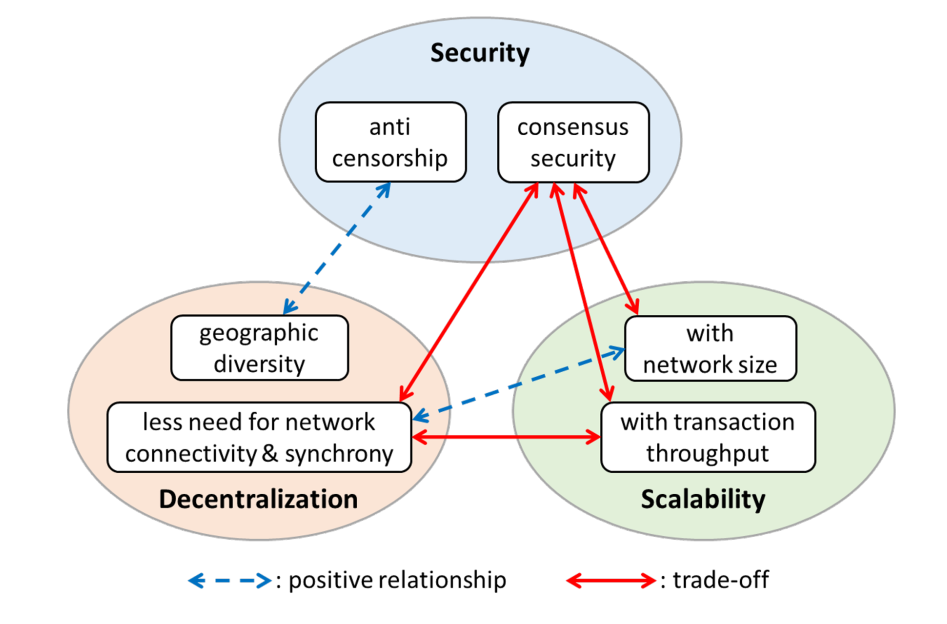
\includegraphics[width=\columnwidth]{trilemma}
  \caption{From \cite{survey-dist-consensus}, the blockchain consensus trilemma and its inner relations.}
  \label{fig:trilemma}
\end{figure}

% Subsection text here.

% needed in second column of first page if using \IEEEpubid
%\IEEEpubidadjcol

% An example of a floating figure using the graphicx package.
% Note that \label must occur AFTER (or within) \caption.
% For figures, \caption should occur after the \includegraphics.
% Note that IEEEtran v1.7 and later has special internal code that
% is designed to preserve the operation of \label within \caption
% even when the captionsoff option is in effect. However, because
% of issues like this, it may be the safest practice to put all your
% \label just after \caption rather than within \caption{}.
%
% Reminder: the "draftcls" or "draftclsnofoot", not "draft", class
% option should be used if it is desired that the figures are to be
% displayed while in draft mode.
%
%\begin{figure}[!t]
%\centering
%\includegraphics[width=2.5in]{myfigure}
% where an .eps filename suffix will be assumed under latex, 
% and a .pdf suffix will be assumed for pdflatex; or what has been declared
% via \DeclareGraphicsExtensions.
%\caption{Simulation results for the network.}
%\label{fig_sim}
%\end{figure}

% Note that the IEEE typically puts floats only at the top, even when this
% results in a large percentage of a column being occupied by floats.


% An example of a double column floating figure using two subfigures.
% (The subfig.sty package must be loaded for this to work.)
% The subfigure \label commands are set within each subfloat command,
% and the \label for the overall figure must come after \caption.
% \hfil is used as a separator to get equal spacing.
% Watch out that the combined width of all the subfigures on a 
% line do not exceed the text width or a line break will occur.
%
%\begin{figure*}[!t]
%\centering
%\subfloat[Case I]{\includegraphics[width=2.5in]{box}%
%\label{fig_first_case}}
%\hfil
%\subfloat[Case II]{\includegraphics[width=2.5in]{box}%
%\label{fig_second_case}}
%\caption{Simulation results for the network.}
%\label{fig_sim}
%\end{figure*}
%
% Note that often IEEE papers with subfigures do not employ subfigure
% captions (using the optional argument to \subfloat[]), but instead will
% reference/describe all of them (a), (b), etc., within the main caption.
% Be aware that for subfig.sty to generate the (a), (b), etc., subfigure
% labels, the optional argument to \subfloat must be present. If a
% subcaption is not desired, just leave its contents blank,
% e.g., \subfloat[].


% An example of a floating table. Note that, for IEEE style tables, the
% \caption command should come BEFORE the table and, given that table
% captions serve much like titles, are usually capitalized except for words
% such as a, an, and, as, at, but, by, for, in, nor, of, on, or, the, to
% and up, which are usually not capitalized unless they are the first or
% last word of the caption. Table text will default to \footnotesize as
% the IEEE normally uses this smaller font for tables.
% The \label must come after \caption as always.
%
%\begin{table}[!t]
%% increase table row spacing, adjust to taste
%\renewcommand{\arraystretch}{1.3}
% if using array.sty, it might be a good idea to tweak the value of
% \extrarowheight as needed to properly center the text within the cells
%\caption{An Example of a Table}
%\label{table_example}
%\centering
%% Some packages, such as MDW tools, offer better commands for making tables
%% than the plain LaTeX2e tabular which is used here.
%\begin{tabular}{|c||c|}
%\hline
%One & Two\\
%\hline
%Three & Four\\
%\hline
%\end{tabular}
%\end{table}


% Note that the IEEE does not put floats in the very first column
% - or typically anywhere on the first page for that matter. Also,
% in-text middle ("here") positioning is typically not used, but it
% is allowed and encouraged for Computer Society conferences (but
% not Computer Society journals). Most IEEE journals/conferences use
% top floats exclusively. 
% Note that, LaTeX2e, unlike IEEE journals/conferences, places
% footnotes above bottom floats. This can be corrected via the
% \fnbelowfloat command of the stfloats package.

% \section{Conclusion}
% The conclusion goes here.

% if have a single appendix:
%\appendix[Proof of the Zonklar Equations]
% or
%\appendix  % for no appendix heading
% do not use \section anymore after \appendix, only \section*
% is possibly needed

% use appendices with more than one appendix
% then use \section to start each appendix
% you must declare a \section before using any
% \subsection or using \label (\appendices by itself
% starts a section numbered zero.)
%


% \appendices
% \section{Proof of the First Zonklar Equation}
% Appendix one text goes here.

% % you can choose not to have a title for an appendix
% % if you want by leaving the argument blank
% \section{}
% Appendix two text goes here.


% % use section* for acknowledgment
% \section*{Acknowledgment}


% The authors would like to thank...


% Can use something like this to put references on a page
% by themselves when using endfloat and the captionsoff option.
\ifCLASSOPTIONcaptionsoff
  \newpage
\fi



% trigger a \newpage just before the given reference
% number - used to balance the columns on the last page
% adjust value as needed - may need to be readjusted if
% the document is modified later
%\IEEEtriggeratref{8}
% The "triggered" command can be changed if desired:
%\IEEEtriggercmd{\enlargethispage{-5in}}

% references section

% can use a bibliography generated by BibTeX as a .bbl file
% BibTeX documentation can be easily obtained at:
% http://mirror.ctan.org/biblio/bibtex/contrib/doc/
% The IEEEtran BibTeX style support page is at:
% http://www.michaelshell.org/tex/ieeetran/bibtex/

%
% <OR> manually copy in the resultant .bbl file
% set second argument of \begin to the number of references
% (used to reserve space for the reference number labels box)

\bibliography{bib}{}
\bibliographystyle{unsrt}

% biography section
% 
% If you have an EPS/PDF photo (graphicx package needed) extra braces are
% needed around the contents of the optional argument to biography to prevent
% the LaTeX parser from getting confused when it sees the complicated
% \includegraphics command within an optional argument. (You could create
% your own custom macro containing the \includegraphics command to make things
% simpler here.)
%\begin{IEEEbiography}[{\includegraphics[width=1in,height=1.25in,clip,keepaspectratio]{mshell}}]{Michael Shell}
% or if you just want to reserve a space for a photo:

% \begin{IEEEbiography}{Michael Shell}
% Biography text here.
% \end{IEEEbiography}

% % if you will not have a photo at all:
% \begin{IEEEbiographynophoto}{John Doe}
% Biography text here.
% \end{IEEEbiographynophoto}

% insert where needed to balance the two columns on the last page with
% biographies
%\newpage

% \begin{IEEEbiographynophoto}{Jane Doe}
% Biography text here.
% \end{IEEEbiographynophoto}

% You can push biographies down or up by placing
% a \vfill before or after them. The appropriate
% use of \vfill depends on what kind of text is
% on the last page and whether or not the columns
% are being equalized.

%\vfill

% Can be used to pull up biographies so that the bottom of the last one
% is flush with the other column.
%\enlargethispage{-5in}



% that's all folks
\end{document}


